\documentclass{scrartcl}\usepackage[]{graphicx}\usepackage[]{color}
%% maxwidth is the original width if it is less than linewidth
%% otherwise use linewidth (to make sure the graphics do not exceed the margin)
\makeatletter
\def\maxwidth{ %
  \ifdim\Gin@nat@width>\linewidth
    \linewidth
  \else
    \Gin@nat@width
  \fi
}
\makeatother

\definecolor{fgcolor}{rgb}{0.345, 0.345, 0.345}
\newcommand{\hlnum}[1]{\textcolor[rgb]{0.686,0.059,0.569}{#1}}%
\newcommand{\hlstr}[1]{\textcolor[rgb]{0.192,0.494,0.8}{#1}}%
\newcommand{\hlcom}[1]{\textcolor[rgb]{0.678,0.584,0.686}{\textit{#1}}}%
\newcommand{\hlopt}[1]{\textcolor[rgb]{0,0,0}{#1}}%
\newcommand{\hlstd}[1]{\textcolor[rgb]{0.345,0.345,0.345}{#1}}%
\newcommand{\hlkwa}[1]{\textcolor[rgb]{0.161,0.373,0.58}{\textbf{#1}}}%
\newcommand{\hlkwb}[1]{\textcolor[rgb]{0.69,0.353,0.396}{#1}}%
\newcommand{\hlkwc}[1]{\textcolor[rgb]{0.333,0.667,0.333}{#1}}%
\newcommand{\hlkwd}[1]{\textcolor[rgb]{0.737,0.353,0.396}{\textbf{#1}}}%
\let\hlipl\hlkwb

\usepackage{framed}
\makeatletter
\newenvironment{kframe}{%
 \def\at@end@of@kframe{}%
 \ifinner\ifhmode%
  \def\at@end@of@kframe{\end{minipage}}%
  \begin{minipage}{\columnwidth}%
 \fi\fi%
 \def\FrameCommand##1{\hskip\@totalleftmargin \hskip-\fboxsep
 \colorbox{shadecolor}{##1}\hskip-\fboxsep
     % There is no \\@totalrightmargin, so:
     \hskip-\linewidth \hskip-\@totalleftmargin \hskip\columnwidth}%
 \MakeFramed {\advance\hsize-\width
   \@totalleftmargin\z@ \linewidth\hsize
   \@setminipage}}%
 {\par\unskip\endMakeFramed%
 \at@end@of@kframe}
\makeatother

\definecolor{shadecolor}{rgb}{.97, .97, .97}
\definecolor{messagecolor}{rgb}{0, 0, 0}
\definecolor{warningcolor}{rgb}{1, 0, 1}
\definecolor{errorcolor}{rgb}{1, 0, 0}
\newenvironment{knitrout}{}{} % an empty environment to be redefined in TeX

\usepackage{alltt}
\author{Medicus,Oberreiter,Hilgart}

\usepackage{babel,amsmath, amsthm}
\usepackage{hyperref}
\hypersetup{
    colorlinks=true, %set true if you want colored links
    linktoc=all,     %set to all if you want both sections and subsections linked
    linkcolor=blue,  %choose some color if you want links to stand out
}
\IfFileExists{upquote.sty}{\usepackage{upquote}}{}
\begin{document}

\title{QAD-Package}

\maketitle

\tableofcontents

\section{Introduction}

The \textit{"Quantification of Asymmetric Dependence"} package introduces a copula-based dependency measure capable of detecting and depicting asymmetry.

It does so, by constructing the empirical copula from a given bivariate sample and aggregating it to the smooth empirical checkerboard copula, which is used as a strongly consistent estimate for the dependency measure used.

\section{qad}

\subsection{Description}

Quantifies the (asymmetric) dependence structure between two random variables $X$ and $Y$.

\subsection{Arguments}
qad(x,\dots)

\begin{itemize}
  \item $x$: either a data.frame containing columns of observations of two random variables or a vector containing the observations of one.
  \item $y$: if $x$ is not a data.frame of two columns, a vector containing the observations of the second random variable.
  \item $resolution$: an integer indicating the number of strips for the checkerboard aggregation. Default = NULL uses the optimal resolution.
  \item $permutation$: a logical indicating whether a permutated p-value is computed.
  \item $nperm$: an integer indicating the number of permutation runs.
\end{itemize}

\subsection{Value}
qad returns an object of class qad containing the following components:

\begin{itemize}
  \item $data$: a data.frame containing the input data.
  \item $results$: a data.frame containing the results of the dependence measures.
  \item $mass\textunderscore matrix$: a matrix containing the mass distribution of the empirical checkerboard copula.
  \item $resolution$: an integer containing the used resolution of the checkerboard aggregation.
\end{itemize}

\subsection{Examples}
\begin{knitrout}
\definecolor{shadecolor}{rgb}{0.969, 0.969, 0.969}\color{fgcolor}\begin{kframe}


{\ttfamily\noindent\color{warningcolor}{\#\# Warning: package 'qad' was built under R version 3.5.3}}\end{kframe}
\end{knitrout}

\begin{knitrout}
\definecolor{shadecolor}{rgb}{0.969, 0.969, 0.969}\color{fgcolor}\begin{kframe}
\begin{alltt}
\hlstd{n} \hlkwb{=} \hlnum{200}
\hlstd{x} \hlkwb{=} \hlkwd{runif}\hlstd{(n,}\hlopt{-}\hlnum{2}\hlstd{,}\hlnum{4}\hlstd{)}
\hlstd{y} \hlkwb{=} \hlkwd{sin}\hlstd{(x}\hlopt{^}\hlnum{2}\hlstd{)}
\hlstd{df} \hlkwb{=} \hlkwd{data.frame}\hlstd{(x,y)}
\hlstd{model} \hlkwb{=} \hlkwd{qad}\hlstd{(df,} \hlkwc{print} \hlstd{=} \hlnum{FALSE}\hlstd{,} \hlkwc{permutation} \hlstd{=} \hlnum{TRUE}\hlstd{)}
\hlstd{model}\hlopt{$}\hlstd{results}
\end{alltt}
\begin{verbatim}
##                        coef p.values
## 1        q(x1,x2) 0.7090350        0
## 2        q(x2,x1) 0.4169353        0
## 3 mean.dependence 0.5629851        0
## 4 asymmetry       0.2920997        0
\end{verbatim}
\end{kframe}
\end{knitrout}

\section{pairwise.qad}
Computes the function qad() for each pair of columns in the given data frame and returns a list of corresponding qad objects.

\section{heatmap.qad}
The pairwise computated dependency measure as output from the pairwise.qad() function, are illustrated by a heatmap.

\subsection{Arguments}

\begin{itemize}
  \item $pw\textunderscore qad$: output of the function pairwise.qad().
  \item $select$: a character indicating which dependence value is plotted. Options are c("dependence","mean.dependence", "asymmetry").
  \item $fontsize$: a numeric specifying the font size of the values.
  \item $significance$: a logical indicating whether significant values - with respect to the permutatedp.values - are marked with a star.
  \item $sign.level$: numeric value indicating the significance level.
  \item $scale$: character indicating whether the heatmap uses a relative or absolute scale.  Op-tions are "rel" or "abs" (default).
\end{itemize}

\subsection{Example}
\begin{knitrout}
\definecolor{shadecolor}{rgb}{0.969, 0.969, 0.969}\color{fgcolor}\begin{kframe}
\begin{alltt}
  \hlkwd{load}\hlstd{(}\hlkwd{url}\hlstd{(}\hlstr{"http://www.trutschnig.net/RTR.RData"}\hlstd{))}
  \hlstd{df} \hlkwb{=} \hlstd{RTR[}\hlkwd{sample}\hlstd{(}\hlkwd{nrow}\hlstd{(RTR),}\hlnum{1000}\hlstd{),}
           \hlkwd{c}\hlstd{(}\hlstr{'long'}\hlstd{,}\hlstr{'lat'}\hlstd{,}\hlstr{'rtr_speed_dl'}\hlstd{,}\hlstr{'rtr_speed_ul'}\hlstd{)]}
  \hlstd{model} \hlkwb{=} \hlkwd{pairwise.qad}\hlstd{(df)}
\end{alltt}
\begin{verbatim}
## [1] "Process..."
## [1] "Process: 1 / 4"
## [1] "Process: 2 / 4"
## [1] "Process: 3 / 4"
\end{verbatim}
\begin{alltt}
  \hlkwd{heatmap.qad}\hlstd{(model)}
\end{alltt}
\end{kframe}
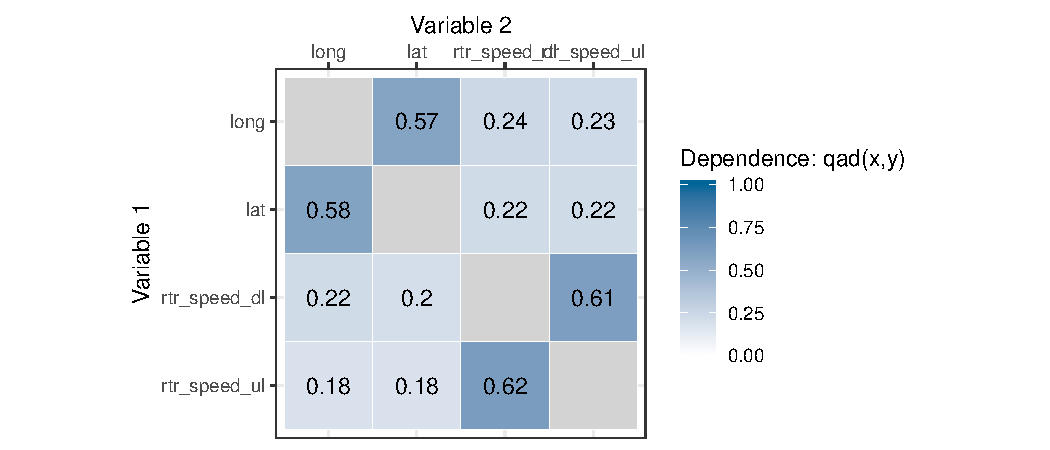
\includegraphics[width=\maxwidth]{figure/unnamed-chunk-3-1} 

\end{knitrout}

\section{cci}

An approximated confidence interval for the dependence measure qad(x,y) for independent random variables . cci() can thus be used to test for independence

\subsection{Arguments}

\begin{itemize}
  \item $n$: and integer indicating the sample size
  \item $alternative$: character string, whether a "one.sided" (default), or "two.sided" confidence intervall is constructed.
\end{itemize}

\subsection{Example}

\begin{knitrout}
\definecolor{shadecolor}{rgb}{0.969, 0.969, 0.969}\color{fgcolor}\begin{kframe}
\begin{alltt}
\hlstd{c} \hlkwb{=} \hlkwd{cci}\hlstd{(n,} \hlkwc{alternative} \hlstd{=} \hlstr{"one.sided"}\hlstd{)}

\hlstd{x} \hlkwb{=} \hlkwd{runif}\hlstd{(n,}\hlopt{-}\hlnum{2}\hlstd{,}\hlnum{4}\hlstd{)}
\hlstd{y} \hlkwb{=} \hlkwd{sin}\hlstd{(x}\hlopt{^}\hlnum{2}\hlstd{)}
\hlstd{df} \hlkwb{=} \hlkwd{data.frame}\hlstd{(x,y)}
\hlstd{model} \hlkwb{=} \hlkwd{qad}\hlstd{(df,}\hlkwc{print}\hlstd{=}\hlnum{FALSE}\hlstd{)}

\hlkwa{if}\hlstd{(}\hlkwd{coef}\hlstd{(model,} \hlkwc{select} \hlstd{=} \hlstr{'q(x1,x2)'}\hlstd{)} \hlopt \hlstd{c)\{}
 \hlkwd{print}\hlstd{(}\hlstr{'Accept H0'}\hlstd{)}
\hlstd{\}}\hlkwa{else}\hlstd{\{}
 \hlkwd{print}\hlstd{(}\hlstr{'Reject H0'}\hlstd{)}
\hlstd{\}}
\end{alltt}
\begin{verbatim}
## [1] "Reject H0"
\end{verbatim}
\end{kframe}
\end{knitrout}


\end{document}
